\documentclass[12pt, fleqn]{beamer}
\usepackage[utf8]{inputenc}
\usepackage[T2A]{fontenc}
\usepackage{amssymb, amsmath, mathrsfs, amsthm}
\usepackage[russian]{babel}
\usepackage{graphicx}
\usepackage{indentfirst}
\usepackage{algorithm}
\usepackage{algpseudocode}
\usetheme{Warsaw}
%\addto\captionsrussian{\renewcommand{\figurename}{Рисунок}}
\title{Конференция Ломоносов-2022}
\subtitle{Методы аугментации аудиоданных}
\author{Лукьянов Павел Александрович}
\institute {\normalsize
Научный руководитель: \\
д.ф-м.н., профессор\\
Дьяконов Александр Геннадьевич \normalsize
}
\date{Москва, 2022} 
\begin{document}% начало презентации
	
\begin{frame}
	\titlepage
\end{frame}

\begin{frame}{Аугментация аудиоданных}
	\begin{figure}[h]
		\centering
		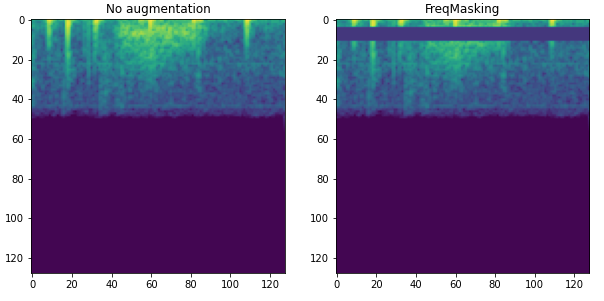
\includegraphics[scale=0.7]{6_0.png}
		\caption{FreqMasking}
		\label{ris:image4}
	\end{figure}
\end{frame}

\begin{frame}{SwapVerticalStripes}
	$t \sim U\{0, T\}, t_1 \sim U\{t, \text{TimeSize} - 1 - t\}$, 
	\newline $t_2 \sim U\{t, \text{TimeSize} - 1 - t\}, |t_1 - t_2| >= t $.  \newline 
	$S[:, t_1: t_1 + t - 1] \leftrightarrow S[:, t_2 : t_2 + t - 1]$
    \begin{figure}[ht!]
    	\center{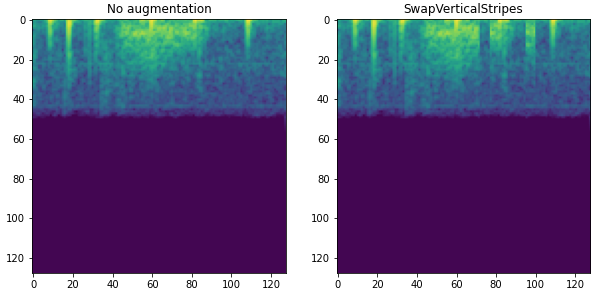
\includegraphics[scale=0.6]{3_0.png}}
    	\caption{SwapVerticalStripes}
    	\label{fig:i3}
    \end{figure}
\end{frame}

\begin{frame}{Эксперименты}
	\begin{table}[ht!]
    \centering
	\begin{tabular}{| l | l | c |}
    	\hline
	    Метод аугментации & resnet18 & resnet50 \\ \hline
	    Аугментация отсутствует  & 81.98 $\pm$ 2.34 & 82.23 $\pm$ 2.4 \\ \hline
	    SwapVerticalStripes & 83.2 $\pm$ 1.3 & 83.65 $\pm$ 1.07 \\ \hline
	\end{tabular}
	\caption{Результаты экспериментов (Heartbeat Sounds) с предлагаемым методом аугментации SwapVerticalStripes}
	\label{table:lukianov_pavel_t1}
\end{table}

\begin{table}[ht!]
    \centering
	\begin{tabular}{| l | l | c |}
    	\hline
	    Метод аугментации & resnet18 & resnet50 \\ \hline
	    Аугментация отсутствует  & 74.3 $\pm$ 3.03 & 73.0 $\pm$ 3.24 \\ \hline
	    SwapVerticalStripes & 76.6 $\pm$ 2.67 & 75.6 $\pm$ 3.68 \\ \hline
	\end{tabular}
	\caption{Результаты экспериментов (GTZAN) с предлагаемым методом аугментации SwapVerticalStripes}
	\label{table:lukianov_pavel_t2}
\end{table}
\end{frame}

\begin{frame}{Алгоритм применения методов аугментации}

\algrenewcommand\algorithmicdo{\textbf{выполнять}}
\algrenewcommand\algorithmicfor{\textbf{Цикл}}
\algrenewtext{EndFor}{\textbf{Конец цикла}}

\begin{algorithm}[H]
    \caption{Предлагаемый алгоритм}\label{alg:Alg1}
    \begin{algorithmic}
    \State $\text{Augmentations} = \{Augment_1, Augment_2, ..., Augment_n\}$ --- заданный набор аугментаций,
    \State $Augment$ --- случайно выбранная аугментация  из $\text{Augmentations}$,
    \State $(X_{val}, y_{val})$ --- валидационный датасет, 
    \State $(X_{train}, y_{train})$ --- обучающая выборка,
    \State $f$ --- метрика качества,
    \State $M$ --- число эпох обучения нейронной сети
    \For{\textbf{от} $j=0$ \textbf{до} M}
    \State train-шаг с применением $Augment$
    \State вычисление $F_i = f(Augment_i(X_{val}), y_{val}), i = \overline{1,n}$
    \State $Augment = Augment_k$, где $k = argmin_k(F_k)$
    \EndFor
    \end{algorithmic}
\end{algorithm}
\end{frame}


\begin{frame}{Эксперименты}
	\begin{table}[ht!]
    \centering
	\begin{tabular}{| l | l | c |}
    	\hline
	    Метод аугментации & resnet18 & resnet50 \\ \hline
	    Аугментация отсутствует  & 81.98 $\pm$ 2.34 & 82.23 $\pm$ 2.4 \\ \hline
	    RandAugment & 83.1 $\pm$ 0.92 & 84.57 $\pm$ 1.3 \\ \hline
	    Предлагаемый алгоритм & 86.65 $\pm$ 0.67 & 86.75 $\pm$ 0.76 \\ \hline
	\end{tabular}
	\caption{Результаты экспериментов (Heartbeat Sounds) с предлагаемым алгоритмом применения методов аугментации}
	\label{table:lukianov_pavel_t3}
\end{table}

    \begin{table}[ht!]
        \centering
    	\begin{tabular}{| l | l | c |}
        	\hline
    	    Метод аугментации & resnet18 & resnet50 \\ \hline
    	    Аугментация отсутствует  & 74.3 $\pm$ 3.03 & 73.0 $\pm$ 3.24 \\ \hline
    	    RandAugment & 75.0 $\pm$ 2.61 & 74.9 $\pm$ 2.63 \\ \hline
    	    Предлагаемый алгоритм & 76.8 $\pm$ 1.75 & 72.2 $\pm$ 2.8 \\ \hline
    	\end{tabular}
    	\caption{Результаты экспериментов (GTZAN) с предлагаемым алгоритмом применения методов аугментации}
    	\label{table:lukianov_pavel_t4}
    \end{table}
\end{frame}

\begin{frame}{Заключение}
	В процессе выполнения работы получены следующие результаты:
	\begin{itemize}
		\item Предложен и реализован метод аугментации аудиоданных SwapVerticalStripes
		\item Проведены вычислительные эксперименты, показавшие возможную применимость предложенного метода в задаче аудиоклассификации
		\item Предложен и реализован алгоритм применения методов аугментации аудиоданных с выбором конкретного метода аугментации после каждой эпохи
		\item Проведены вычислительные эксперименты, показавшие возможную применимость предложенного алгоритма в задаче аудиоклассификации
	\end{itemize}
\end{frame}

\begin{frame}{Список литературы}
\begin{itemize}
\item \textit{Ekin D. Cubuk, Barret Zoph, Jonathon Shlens, Quoc V. Le}. RandAugment: Practical automated data augmentation with a reduced search space // \textit{arXiv preprint arXiv:1909.13719.} --- 2019.
\item \textit{Bentley, P. and Nordehn, G. and Coimbra, M. and Mannor, S.} The {PASCAL} {C}lassifying {H}eart {S}ounds {C}hallenge 2011 {(CHSC2011)} {R}esults. --- 2011.
\url{http://www.peterjbentley.com/heartchallenge/index.html}
\item \textit{G. Tzanetakis and P. Cook. Musical genre classification of audio signals.}    // IEEE Transactions on Speech and Audio Processing. --- 2002.
\end{itemize}
\end{frame}

\begin{frame}{Список литературы}
\begin{itemize}
\item \textit{Daniel S. Park, William Chan, Yu Zhang, Chung-Cheng Chiu, Barret Zoph, Ekin D. Cubuk, Quoc V. Le}. SpecAugment: A Simple Data Augmentation Method
for Automatic Speech Recognition // \textit{arXiv preprint arXiv:1904.08779.} - 2019.
\item \textit{Kaiming He, Xiangyu Zhang, Shaoqing Ren, Jian Sun.} Deep Residual Learning for Image Recognition // In Proceedings of the IEEE Conference on Computer Vision and Pattern Recognition (CVPR), 2016, pp. 770-778.
\end{itemize}
\end{frame}

\end{document}